\chapter{Imágenes del Sistema Hardware}
\label{anexo:img}
En la Figura \ref{fig:all} se puede ver la placa para la que se ha realizado este \acs{TFG}, conectada a la interfaz de programación y depuración.\\

\begin{figure}[!h]
\begin{center}
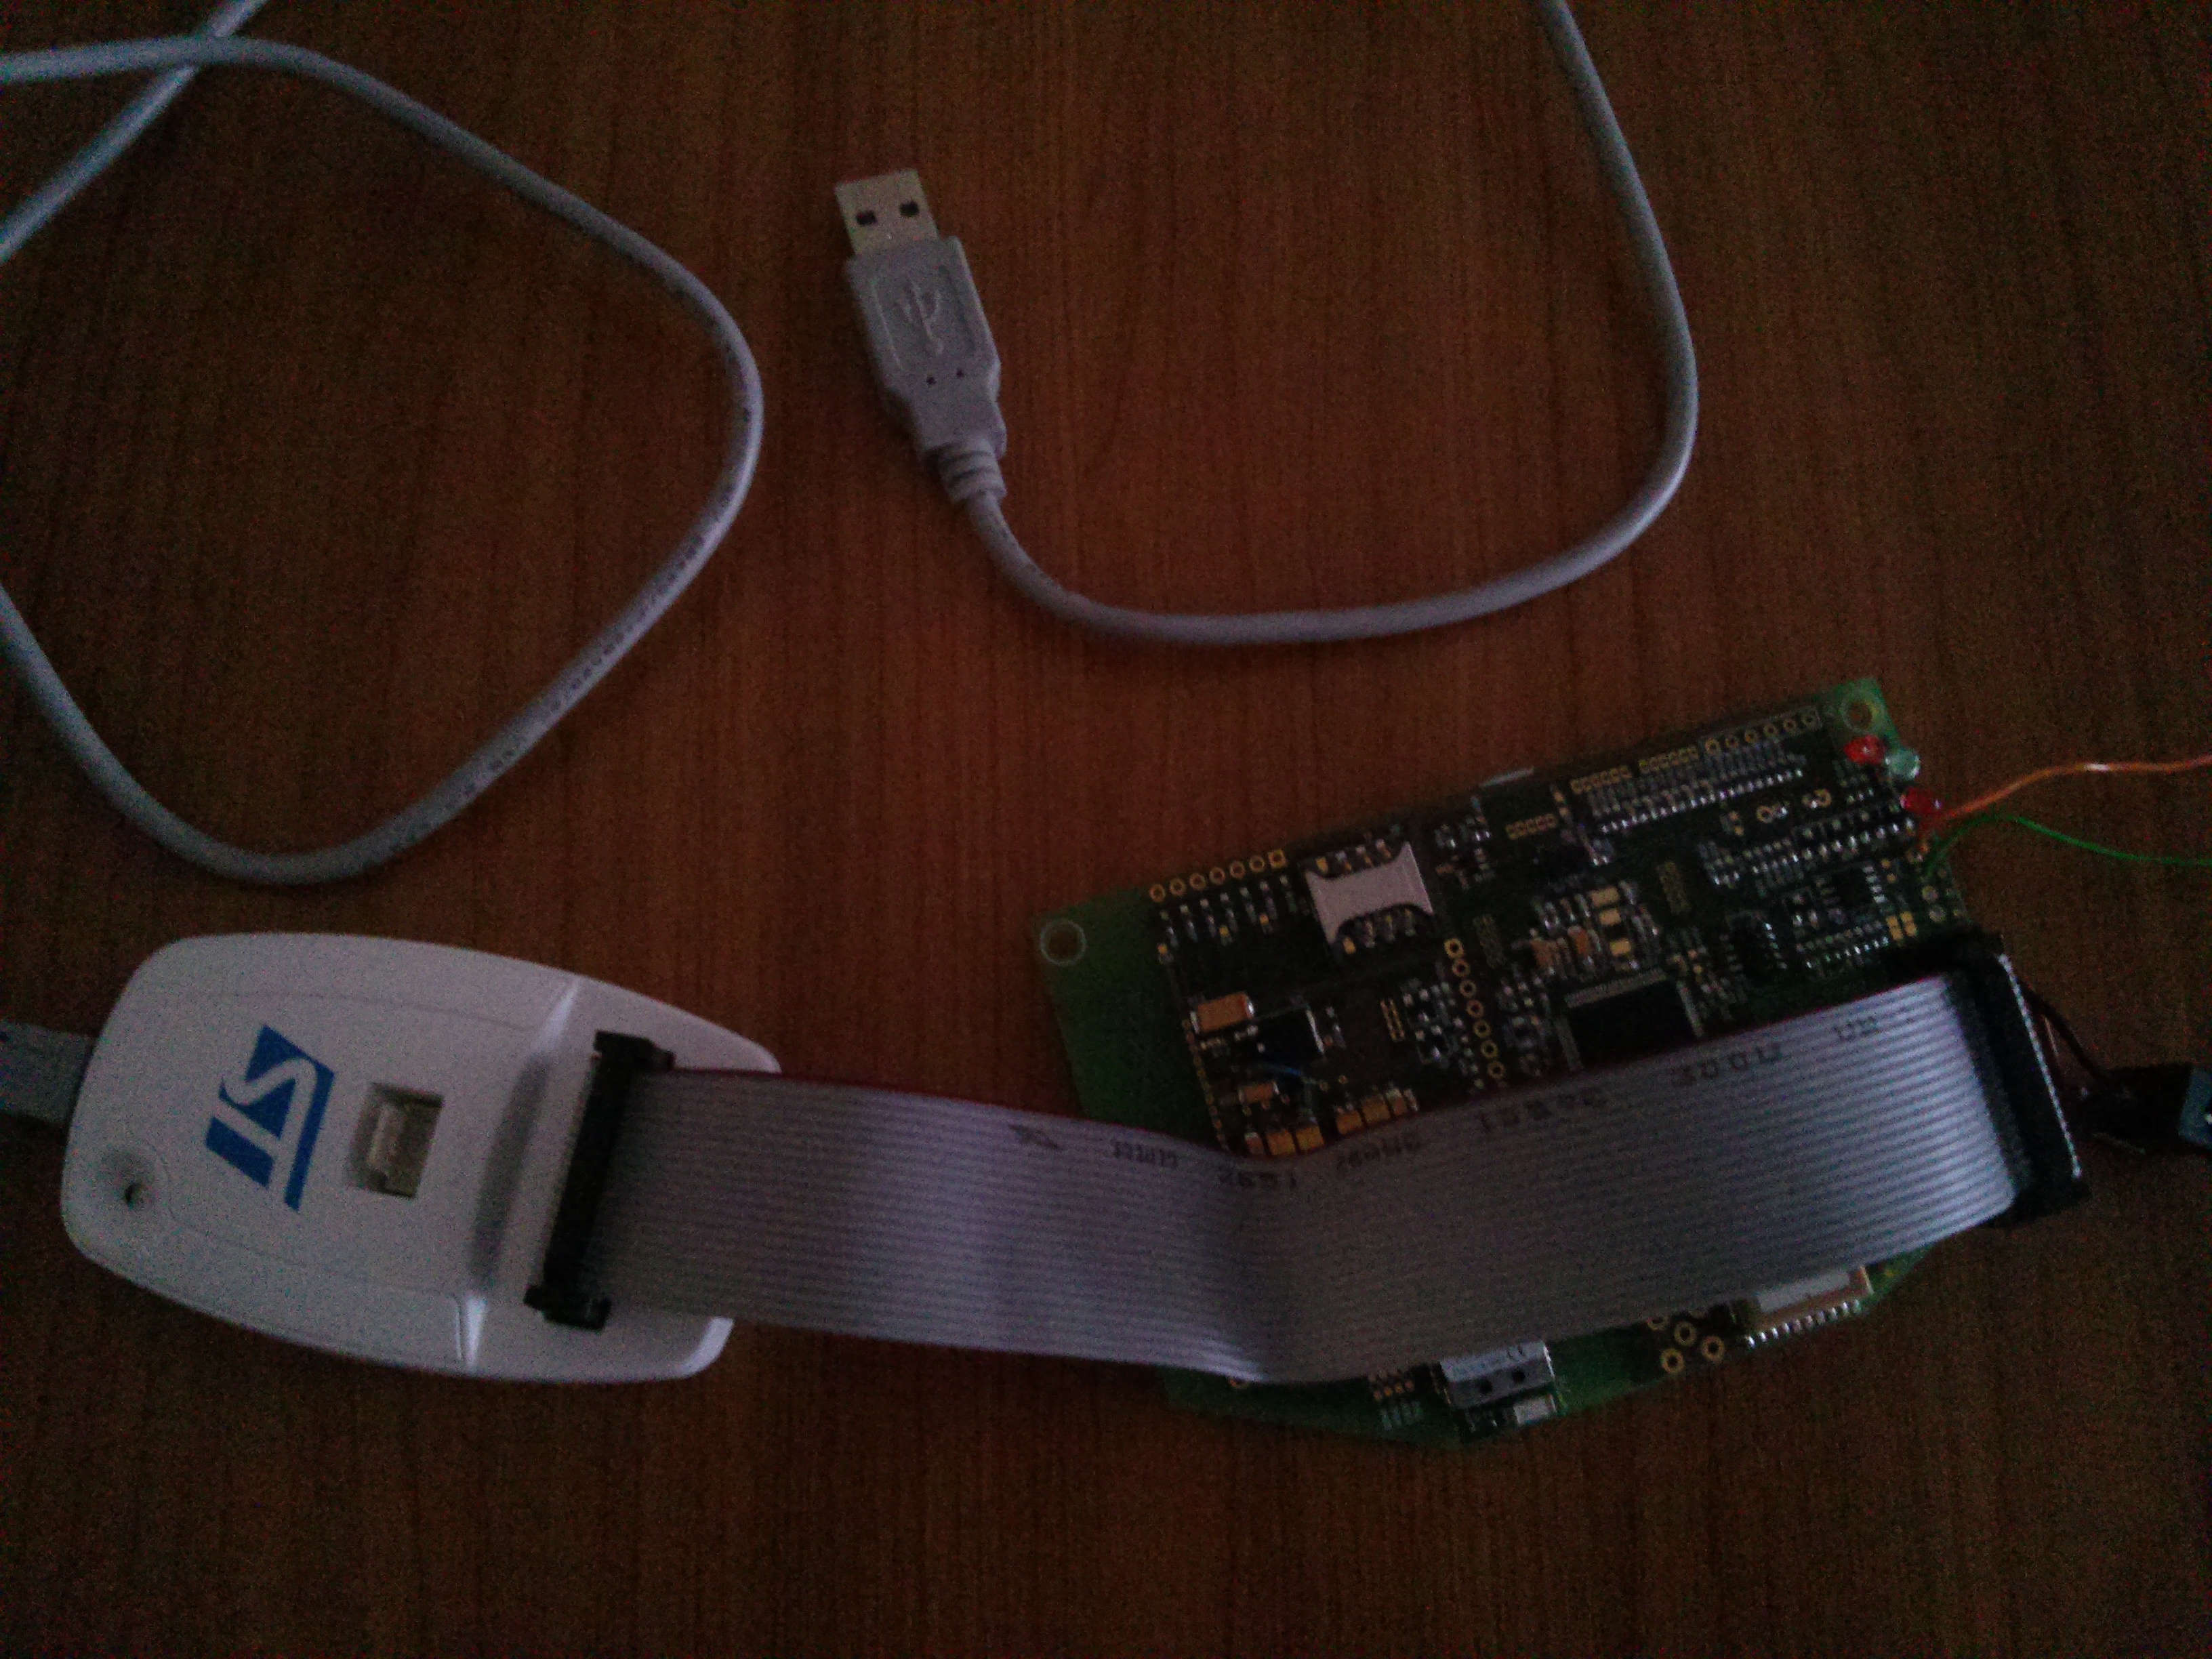
\includegraphics[width=0.8\textwidth]{figs/all.jpg}
\caption{Imagen que muestran todos los componentes hardware del sistema}
\label{fig:all}
\end{center}

En la Figura \ref{fig:frontDiagram} se puede ver un diagrama de los componentes más importantes de la placa sobre una imagen de la misma. Normalmente este tipo de diagramas se realiza sobre un dibujo de la placa, pero de esta forma queda más claro dónde está cada componente.\\

\end{figure}
\begin{figure}[!h]
\begin{center}
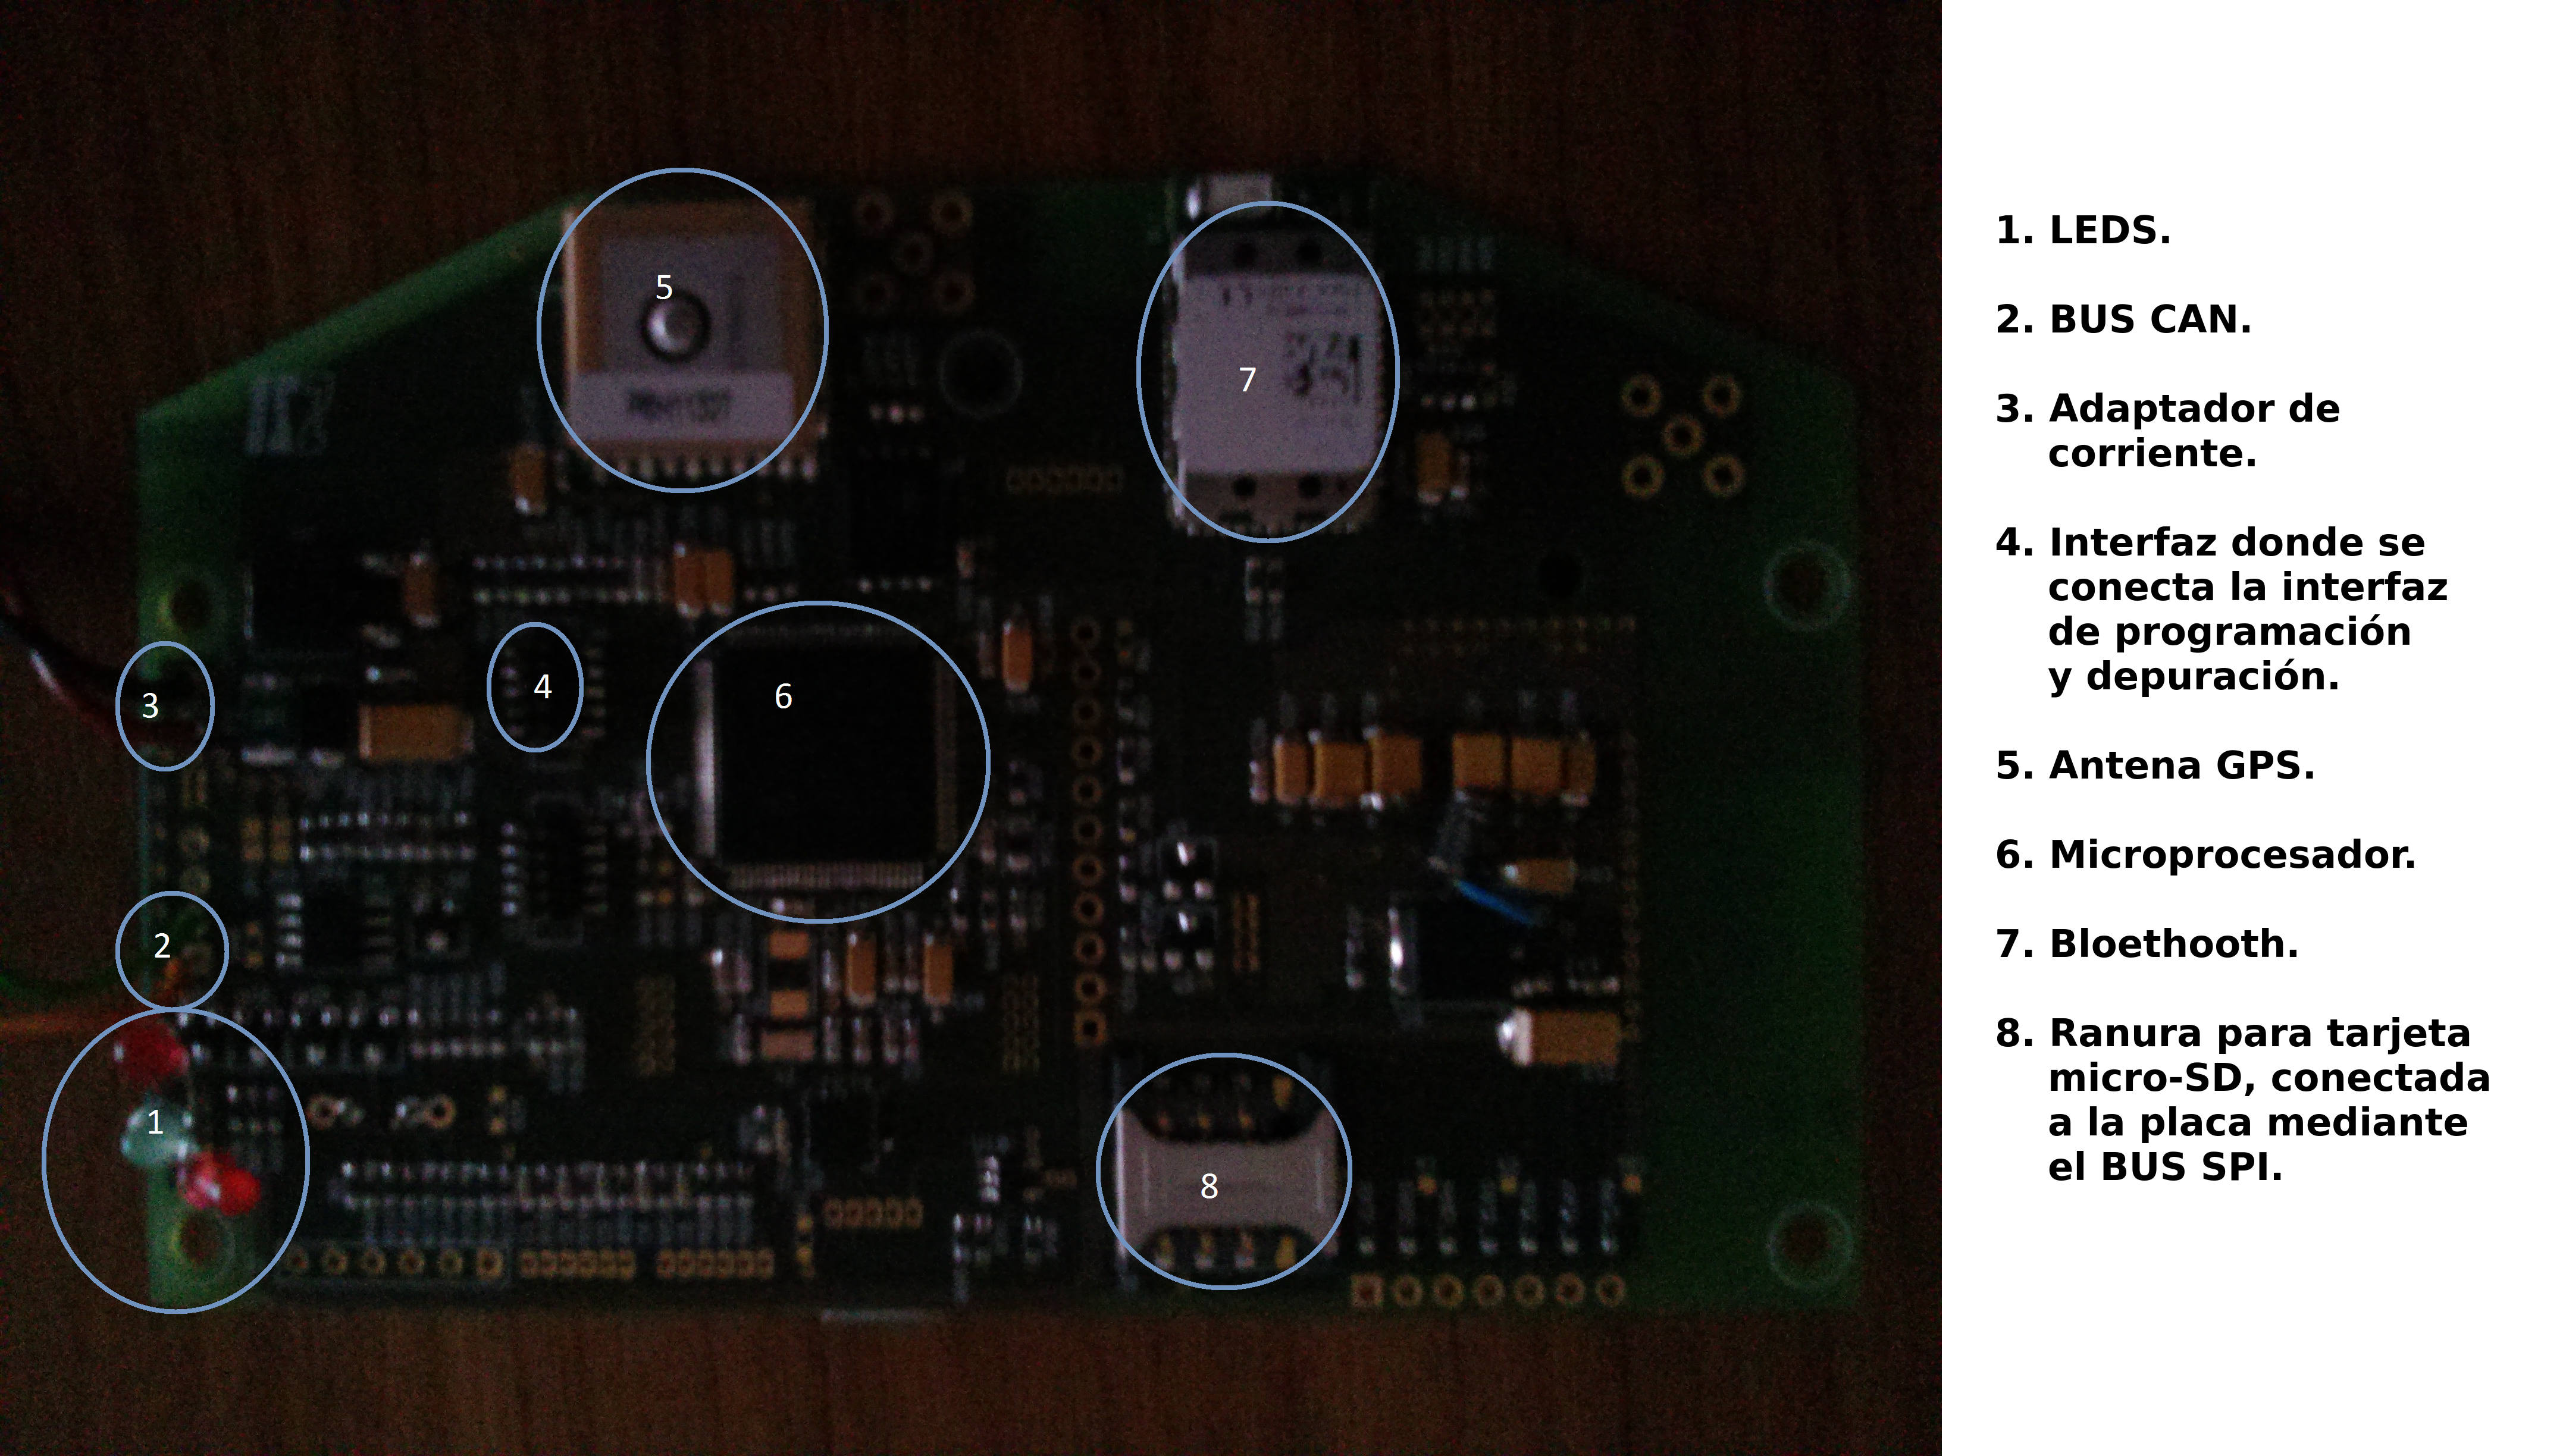
\includegraphics[width=0.8\textwidth]{figs/frontDiagram.jpg}
\caption{Diagrama de componentes sobre una imagen de la placa}
\label{fig:frontDiagram}
\end{center}
\end{figure}

